\subsection*{2.1}
%    1. Build a common-source MOS amplifier as shown below using BS170 transistor.
%Element values: R1 = R2 = 100 k, R3 = R4 = 470 , RL = 1 k, C1 = 1 µF, C2 = 100 µF,
%C3 = 10 µF. Use VDD = 15 V.

    \begin{figure}[h!]
        \centering
        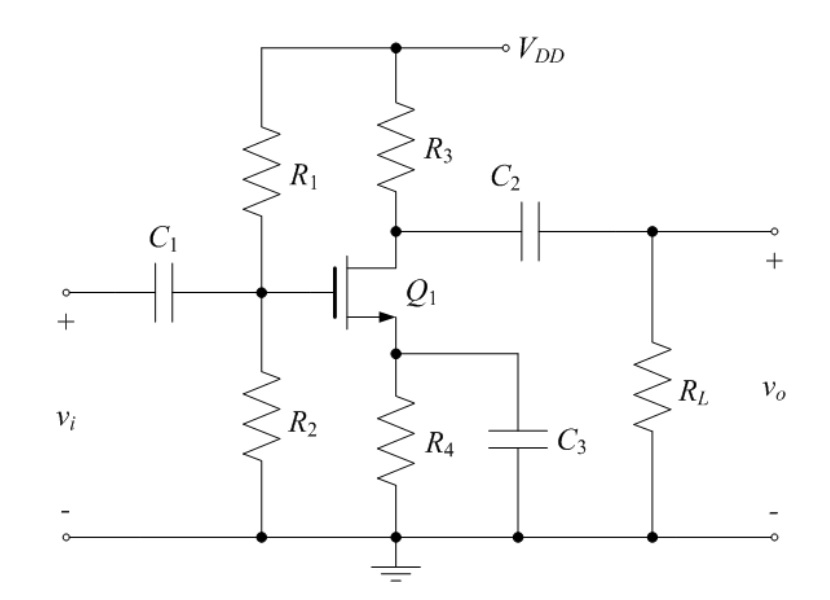
\includegraphics[width=6cm]{circuit_task_2.jpg}
        \captionof{figure}{Circuit built in task 2}
    \end{figure}

\subsection*{2.2}

%2. Use Bode Analyzer to measure the AC characteristic of the amplifier in the frequency
%range 10 Hz to 50 kHz. Use 10 steps per decade and input signal amplitude of 50 mV.
%Find the lower 3dB frequency of the circuit.


\subsection*{2.3}
%3. Determine the following parameters of the circuit (at the frequency 1 kHz): voltage gain,
%input resistance, output resistance. Input signal amplitude should be small, e.g., 50 mV.
%Observe and store the input and output signal waveforms using oscilloscope.


\subsection*{2.4}
% 4. Using the transistor parameters obtained in Task 1, determine the values of gain,
%input/output resistance and the lower 3dB frequency theoretically compare them to the
%values obtained experimentally.